% -*- coding: utf-8 -*-
\documentclass[a4paper,12pt]{article}

% بسته‌های مورد نیاز (بدون xepersian)
\usepackage{amsmath,amssymb,amsthm}
\usepackage[linesnumbered,ruled,vlined]{algorithm2e}
\usepackage{tikz}
\usetikzlibrary{arrows,positioning}
\usepackage[margin=2cm]{geometry}
\usepackage{graphicx}
\usepackage{caption}
\usepackage{float}
\usepackage{adjustbox}

% در انتها بسته‌ی xepersian را اضافه می‌کنیم
\usepackage{xepersian}
\settextfont{XB Zar} % انتخاب فونت فارسی؛ در صورت نیاز می‌توانید فونت دلخواه را انتخاب کنید

% تعریف فرمان \EN به گونه‌ای که داخل محیط ریاضی هم درست کار کند
\newcommand{\EN}[1]{\text{\lr{#1}}}

\newtheorem{definition}{تعریف}[section]
\newtheorem{theorem}{قضیه}[section]
\newtheorem{lemma}{لم}[section]
\newtheorem{example}{مثال}[section]

\title{تشخیص رئوس برشی در گراف با استفاده از \EN{DFS}}
\author{محمد جواد عبدالهی}
\date{}

\begin{document}
	
	\maketitle
	
	\section{تعاریف اولیه}
	
	\begin{definition}[\EN{DFNum}]
		در یک جستجوی عمق‌اول \EN{DFS} روی گراف
		\(G=(V,E)\)
		به هر رأس
		\(u\in V\)
		عددی به نام
		\(\EN{DFNum}(u)\)
		اختصاص داده می‌شود که نشان‌دهنده‌ی ترتیب بازدید
		\(u\)
		در طی \EN{DFS} است.
	\end{definition}
	
	\begin{definition}[\EN{Low}]
		برای هر رأس
		\(u\in V\)
		مقدار
		\(\EN{Low}(u)\)
		به صورت زیر تعریف می‌شود:
		\[
		\EN{Low}(u)
		=\min\Bigl\{\,
		\EN{DFNum}(u),
		\,\min_{v\in\text{فرزندان }u}\EN{Low}(v),
		\,\min\{\EN{DFNum}(w)\mid (u,w) \text{ یک یال برگشتی است}\}
		\Bigr\}.
		\]
		
		این مقدار نشان‌دهنده‌ی آن است که از طریق
		\(u\)
		یا زیردرخت
		\(u\)
		(با استفاده از یال‌های درختی یا برگشتی)،
		به کدام عدد کمترین
		\(\EN{DFNum}\)
		دسترسی وجود دارد.
	\end{definition}
	
	\begin{definition}[رأس برشی]
		یک رأس
		\(u\)
		(به جز ریشه \EN{DFS}) در گراف به عنوان 
		\textbf{رأس برشی \EN{(Articulation Point)}}
		شناخته می‌شود اگر برای حداقل یک فرزند
		\(v\)
		در درخت \EN{DFS} شرط زیر برقرار باشد:
		
		\[
		\EN{Low}(v) \ge \EN{DFNum}(u).
		\]
	
		همچنین، ریشه \EN{DFS} در صورتی رأس برشی است که بیش از یک فرزند داشته باشد.
	\end{definition}
\newpage	
	\section{الگوریتم محاسبه‌ی \EN{DFNum} و \EN{Low}}
	
	در ادامه الگوریتم \EN{DFS} به همراه محاسبه‌ی مقادیر
	\(\EN{DFNum}\)
	و
	\(\EN{Low}\)
	ارائه می‌شود:
	
\begin{latin} 
	\begin{algorithm}[H]
		\caption{Computing \(\text{DFNum}\) and \(\text{Low}\) Using DFS}
		\KwData{A graph \( G = (V, E) \) and a starting vertex \( s \)}
		\KwResult{Arrays \(\text{DFNum}\) and \(\text{Low}\) for every vertex, and the set of articulation points}
		\( \text{time} \gets 0 \)\;
		\ForEach{\( u \in V \)}{
			\( \text{DFNum}[u] \gets 0 \)\;
		}
		\BlankLine
		\SetKwFunction{DFS}{DFS}
		\SetKwProg{Fn}{Function}{:}{}
		\Fn{\DFS{\( u \)}}{
			\( \text{time} \gets \text{time} + 1 \)\;
			\( \text{DFNum}[u] \gets \text{time} \)\;
			\( \text{Low}[u] \gets \text{DFNum}[u] \)\;
			\ForEach{\( v \) neighbor of \( u \)}{
				\eIf{\( \text{DFNum}[v] = 0 \)}{
					\( \text{parent}[v] \gets u \)\;
					\DFS{\( v \)}\;
					\( \text{Low}[u] \gets \min \Big( \text{Low}[u], \text{Low}[v] \Big) \)\;
				}{
					\If{\( v \neq \text{parent}[u] \)}{
						\( \text{Low}[u] \gets \min \Big( \text{Low}[u], \text{DFNum}[v] \Big) \)\;
					}
				}
			}
			\If{\( u \neq \text{root} \)}{
				\ForEach{\( v \) child of \( u \)}{
					\If{\( \text{Low}[v] \geq \text{DFNum}[u] \)}{
						Mark \( u \) as an articulation point\;
					}
				}
			}
		}
		\BlankLine
		\DFS{\( s \)}\;
	\end{algorithm}
\end{latin}
\newpage
	\section{اثبات درستی الگوریتم}
\textbf{حالت اول:} اگر ریشه بیش از یک فرزند داشته باشد، حذف آن باعث جدایی زیر درخت‌های DFS می‌شود.\\[1ex]
\textbf{حالت دوم:} اگر گره \lr{$v$} طوری باشد که هیچ مسیر بازگشتی از راس‌های زیر درخت فرزند مانند \lr{$u$} به \lr{$v$} یا اجدادش وجود نداشته باشد، آنگاه حذف \lr{$v$} باعث جدایی \lr{$u$} و زیر درختش می‌شود.\\[1ex]
در هر دو حالت، گراف به مؤلفه‌های جداگانه‌ای تجزیه می‌شود که نشان می‌دهد \lr{$v$} نقطه محوری است.
	\\اثبات درستی الگوریتم به روش استقرایی:
	
	\begin{itemize}
		\item \textbf{پایه استقرا:}
		اگر یک رأس \(u\) برگ باشد، هیچ فرزندی ندارد.
		بنابراین طبق الگوریتم:
		\[
		\EN{Low}(u)=\EN{DFNum}(u),
		\]
		که مطابق تعریف است.
		
		\item \textbf{فرض استقرا:}
		فرض کنید برای هر رأسی با عمق کمتر از \(u\)،
		مقادیر \(\EN{Low}\) به درستی محاسبه شده‌اند.
		
		\item \textbf{گام استقرا:}
		در هنگام بازگشت از فراخوانی \EN{DFS} روی رأس \(u\)،
		مقدار \(\EN{Low}(u)\) به صورت زیر محاسبه می‌شود:
		
		\[
		\EN{Low}(u)
		=\min\Bigl\{
		\EN{DFNum}(u),
		\,\min_{v\in\text{فرزندان }u}\EN{Low}(v),
		\,\min\{\EN{DFNum}(w)\mid (u,w) \text{ یال برگشتی است}\}
		\Bigr\}.
		\]
		
		با توجه به فرض استقرا، مقادیر \(\EN{Low}\) هر فرزند
		به درستی محاسبه شده و در نتیجه مقدار \(\EN{Low}(u)\)
		نیز مطابق تعریف تعیین می‌شود.
	\end{itemize}
	\section{مثال محاسبه نقاط برشی در گراف بدون جهت}
	
	در این مثال گراف زیر را در نظر می‌گیریم:
	
	\begin{figure}[H]
		\centering
		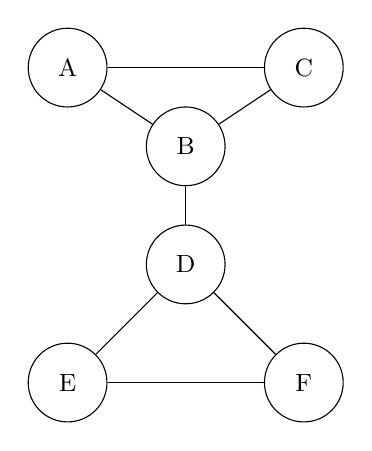
\begin{tikzpicture}[every node/.style={circle,draw,minimum size=10mm,inner sep=1pt}, font=\small]
			
			% Vertices
			\node (A) at (0,2) {A};
			\node (B) at (1.5,1) {B};
			\node (C) at (3,2) {C};
			\node (D) at (1.5,-0.5) {D};
			\node (E) at (0,-2) {E};
			\node (F) at (3,-2) {F};
			
			% Edges
			\draw (A) -- (B);
			\draw (B) -- (C);
			\draw (A) -- (C);
			\draw (B) -- (D);
			\draw (D) -- (E);
			\draw (D) -- (F);
			\draw (E) -- (F);
			
		\end{tikzpicture}
		\caption{گراف بدون‌جهت برای یافتن نقاط برشی}
	\end{figure}
	\begin{figure}[H]
	\centering
		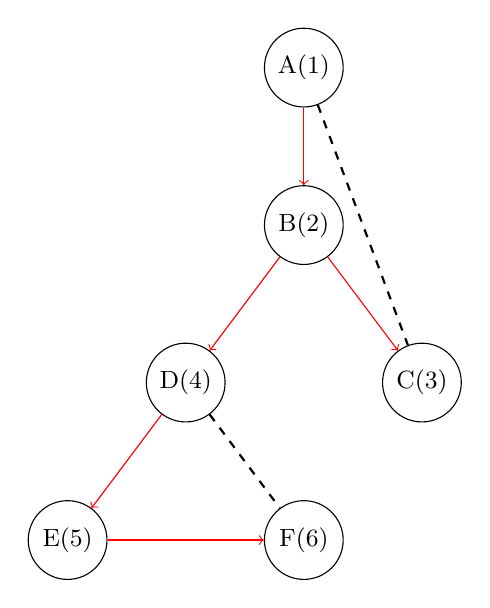
\begin{tikzpicture}[every node/.style={circle,draw,minimum size=10mm,inner sep=1pt}, font=\small]
			
			% Nodes with (DFS, Low) labels
			\node (1) at (0,4) {A(1)};
			\node (2) at (0,2) {B(2)};
			\node (3) at (1.5,0) {C(3)};
			\node (4) at (-1.5,0) {D(4)};
			\node (5) at (-3,-2) {E(5)};
			\node (6) at (0,-2) {F(6)};
			
			% Tree edges (red)
			\draw[red, ->] (1) -- (2);
			\draw[red, ->] (2) -- (3);
			\draw[red, ->] (2) -- (4);
			\draw[red, ->] (4) -- (5);
			\draw[red, ->] (5) -- (6);
			
			% Back edges (black dashed)
			\draw[black, thick, dashed] (1) -- (3);
			\draw[black, thick, dashed] (4) -- (6);
			
		\end{tikzpicture}
		\caption{گراف \EN{DFS}}
	\end{figure}
	\subsection*{مراحل اجرای الگوریتم \EN{DFS} و محاسبه نقاط برشی}
	
	برای اجرای الگوریتم، از رأس \lr{A} شروع می‌کنیم. جدول زیر مقادیر \lr{DFS-Number} و \lr{Low} برای هر رأس را نمایش می‌دهد.
	
\begin{table}[H]
	\centering
	\begin{adjustbox}{center}
		\begin{tabular}{|c|c|c|}
			\hline
			رأس & \EN{DFN} & \EN{Low} \\
			\hline
			A & 1 & 1 \\
			\hline
			B & 2 & 1 \\
			\hline
			C & 3 & 1 \\
			\hline
			D & 4 & 4 \\
			\hline
			E & 5 & 4 \\
			\hline
			F & 6 & 4 \\
			\hline
		\end{tabular}
	\end{adjustbox}
	\caption{مقادیر \EN{DFS} و \EN{Low} برای رأس‌ها}
\end{table}
	
	با توجه به مقادیر \lr{Low} و قوانین زیر، نقاط برشی مشخص می‌شوند:
	
	\begin{itemize}
		\item اگر فرزند \( v \) از \( u \) باشد و \( \text{low}[v] \geq \text{dfs}[u] \)، آنگاه \( u \) رأس برشی است (به‌جز ریشه).
		\item ریشه اگر بیش از یک فرزند در درخت DFS داشته باشد، رأس برشی است.
	\end{itemize}
	مجموعه نقاط برشی در این گراف به‌صورت زیر است:
	
	\[
	\{ B,\ D \}
	\]
	
	\section{نتیجه‌گیری}
	با استفاده از الگوریتم \EN{DFS} و محاسبه‌ی دقیق مقادیر
	\(\EN{DFNum}\) و \(\EN{Low}\)،
	می‌توان رئوس برشی را شناسایی کرد.
	در مثال فوق، حذف B زیردرخت E را جدا می‌کند و حذف C زیردرخت D را؛
	بنابراین B و C رئوس برشی هستند.
	
\end{document}